\begin{frame}{Rete}


\begin{columns}[c]

\column{0.65\textwidth}

\begin{figure}[h!]
\centering

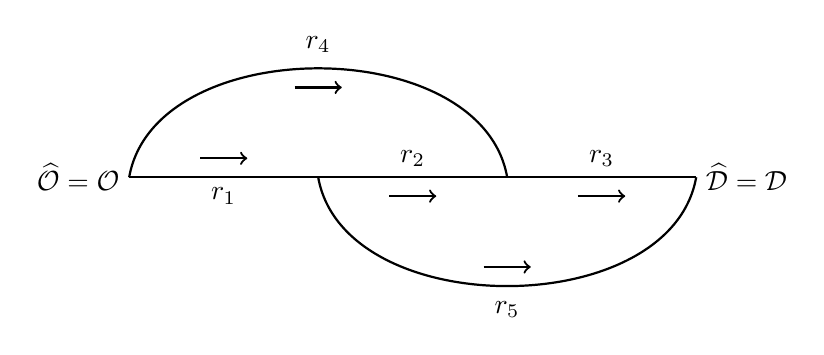
\begin{tikzpicture}[scale=1.2, rotate=-90]

% Nodi principali
\coordinate (A) at (0,0);
\coordinate (B) at (0,6);
\coordinate (Y) at (0,2);
\coordinate (X) at (0,4);

% Segmento principale
\draw[thick] (A) -- (B);

% Arco superiore
\draw[thick]
(B) to[out=-10,in=10] (Y);

% Arco inferiore
\draw[thick]
(A) to[out=170,in=-170] (X);

% Collegamento centrale tratteggiato
\draw[thick, dashed] (Y) -- (X);

% Freccia direzione
\draw[->, thick] (-0.2,0.75) -- (-0.2,1.25);
\draw[->, thick] (0.2,2.75) -- (0.2,3.25);
\draw[->, thick] (0.2,4.75) -- (0.2,5.25);
\draw[->, thick] (-0.95,1.75) -- (-0.95,2.25);
\draw[->, thick] (0.95,3.75) -- (0.95,4.25);

% Etichette
\node[left] at (A) {$\widehat{\mathcal{O}} = \widecheck{\mathcal{O}}$};
\node[right] at (B) {$\widehat{\mathcal{D}} = \widecheck{\mathcal{D}}$};

% Etichette archi
\node at (0.2, 1) {$r_1$};
\node at (-0.2,3) {$r_2$};
\node at (-0.2, 5) {$r_3$};
\node at (-1.4,2) {$r_4$};
\node at (1.4, 4) {$r_5$};

\end{tikzpicture}

\end{figure}

\column{0.35\textwidth}

\textbf{Ipotesi}

\begin{itemize}
    \item Percorso $(r_1, r_2, r_3)$ ad alta viabilità
    \item Strade $r_4$ e $r_5$ scorciatoie nel caso di traffico intenso
    \item La popolazione \textit{hat} conosce le scorciatoie
    \item La popolazione \textit{check} ignora l'esistenza delle scorciatoie
\end{itemize}

\end{columns}

\end{frame}